\scanpage{17}
\figure{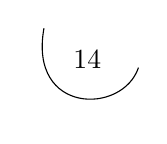
\begin{tikzpicture}[x=1cm,y=1cm]
\node at (0,0) {\mspage{14}};
\draw (-.55,.4) .. controls (-.75,-.7) and (.45,-.7) .. (.65,-.1);
\end{tikzpicture}}
\uline{Corollary} Let $\mathcal E$ be a graded ring, \inserted{\figure{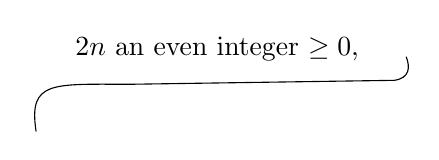
\begin{tikzpicture}[x=1cm,y=1cm]
\node at (0,.35) {$2n$ an even integer $\geq0$,};
\draw (-2.3,-.7) .. controls (-2.4,-.05) and (-2.1,-.1) .. (-1.1,-.1) --(2.25,-.05) .. controls (2.45,-.02) and (2.45,.12) .. (2.4,.25);
\end{tikzpicture}}} and let $L\in\mathcal E^{(2)}$.
If there exists a homomorphism of graded rings
\[
u:\Phi\longrightarrow\mathcal E
\]
such that $u(\mathbf L)=L$, and such that the $u(\boldsymbol\pi_i)=\pi_i$ define the grading of $\mathcal E$ by $(1.3)$, then such a $u$ is uniquely determined, and the $\pi_i$ are uniquely determined, in terms of the graded \inserted{\uline{ring}} structure of $\mathcal E$ by the conditions $(1.1)$ and $(1.3)$.
\inserted{If we are given $\pi_i$ satisfying the conditions \deleted{\unsure{In the absence of the} $\pi_i$},}
\margin{\figure{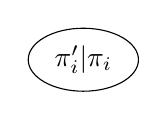
\begin{tikzpicture}\node at (0,0) {$\unsure{\pi'_i|\pi_i}$};\draw (0,0) ellipse (.7cm and .4cm);\end{tikzpicture}}}
the existence of $u$ is then equivalent to : \deleted{the existence} validity, for all $0\leq i\leq n$, of the condition
\[
\text{``}\ \exists w_i\in\mathcal E^{-(2n-2i)}\text{ such that}\quad(w_iL^{n-i}-1)\pi_{\deleted{i}\inserted{2n-i}}\deleted{=0}\text{''}=0,
\]
and \deleted{then} the system of the $\Lambda=u(\boldsymbol\Lambda)$, \deleted{and} $\pi_{i,\alpha}=u(\boldsymbol\pi_{i,\alpha})$ is then characterized (in terms of $L$ and the $\pi_i$) by the equations $(6.14)$.
\margin{Or again : $\exists$ a faithful module $M^*$ over $\mathcal E^*$ such that \unsure{by} \unsure{its|the} grading \unsure{coincides} .... (\unsure{thus this for all}). \deleted{\unsure{If we say}} \unsure{Id of the preceding}.}
From the datum of the $\pi_i$, the existence of $u$ is equivalent to the existence of a faithful \uline{graded} module over $\mathcal E^*$, \deleted{such that} $\mathcal E^*$ (\unsure{defined by the} $\pi_i\in\operatorname{End}(M^*)$), and such that \figure{\begin{tikzpicture}[x=.35cm,y=.35cm,baseline]
\fill (0,0) ellipse (.09 and .045);
\fill (.5,.06) ellipse (.065 and .05);
\fill (.8,.07) ellipse (.07 and .045);
\fill (1.15,.12) ellipse (.09 and .04);
\fill (1.5,.15) ellipse (.055 and .05);
\draw[line width=.8pt] (1.9,.17) .. controls (2.05,.23) and (2.08,.23) .. (2.2,.18);
\draw[line width=.8pt] (2.5,.2)--(2.8,.21);
\fill (4.4,.22) circle (.13);
\end{tikzpicture}}

\uline{Question} If we are \uline{not} given the grading of $\mathcal E$ a priori,
\inserted{\figure{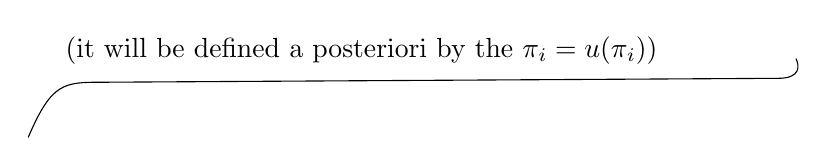
\begin{tikzpicture}[x=1cm,y=1cm]
\node[anchor=west] at (0,.35) {(it will be defined a posteriori by the $\pi_i=u(\boldsymbol\pi_i)$)};
\draw (-.35,-.75) .. controls (-.05,-.05) and (.1,-.05) .. (.6,-.05) --(9.2,.0) .. controls (9.45,.01) and (9.45,.15) .. (9.4,.25);
\end{tikzpicture}}}
would it be true that there is at most one homomorphism $\Phi\longrightarrow\mathcal E$ such that $u(\mathbf L)=L$ !

\figure{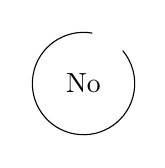
\begin{tikzpicture}\node at (0,0) {No};\draw (80:.65cm) arc[start angle=80,end angle=400,radius=.65cm];\end{tikzpicture}}, already in the case $n=1$, $2n=2$, where there is a basis of $\Phi$ consisting of $\pi_0,\pi_1,\pi_2,L,\Lambda$, and where $\mathbb Z[L]$ is only $\mathbb Z+\mathbb ZL$ ! One must therefore specify at the same time \uline{$L$ and the $\pi_i$}.
\mspage{16}
